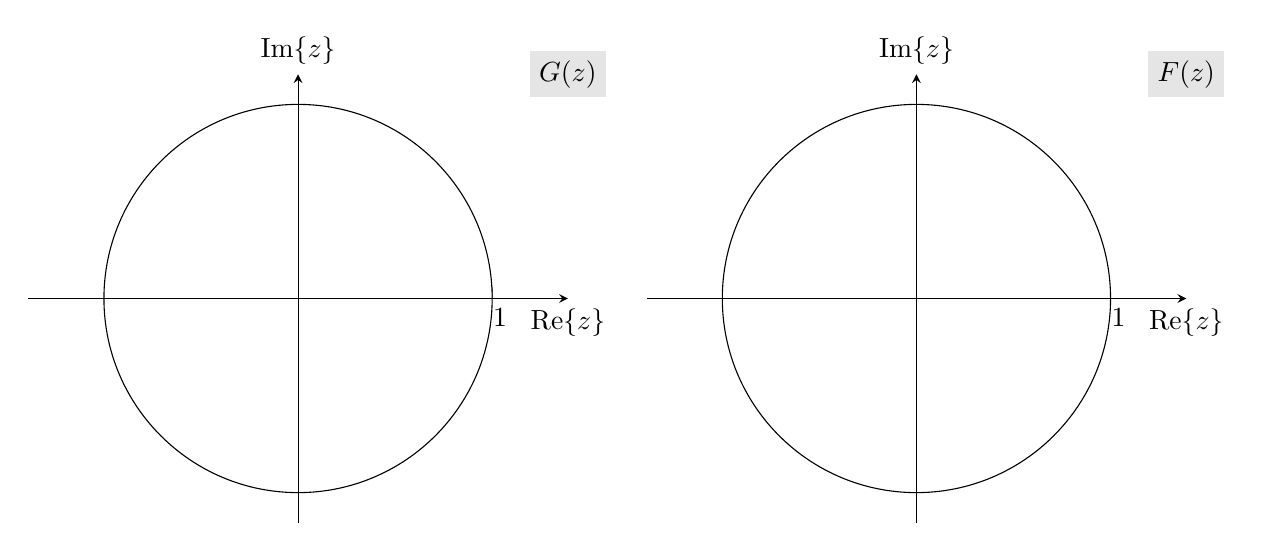
\begin{tikzpicture}
\begin{axis}[
name=plot1,
axis equal,
axis lines*=middle,
enlargelimits = false, clip=true,
xmin=-1.39,
xmax=1.39,
ymin=-1.10,
ymax=1.10,
axis line style={->,>=stealth},
xlabel={$\mathrm{Re}\{z\}$},
ylabel={$\mathrm{Im}\{z\}$},
every axis x label/.style={
at={(ticklabel* cs:1)},
anchor=north,
},
every axis y label/.style={
at={(ticklabel* cs:1)},
anchor=south,
},
xtick=1, ytick=\empty,
xticklabel style={xshift=0.1cm},
every outer y axis line/.append style={white!15!black},
every y tick label/.append style={font=\color{white!15!black}},
legend style={draw=white!15!black,fill=white,legend cell align=left}]
\draw (axis cs:0,0) circle [black!50, dashed, line width=2pt, radius=1];
\if\SOLUTIONS1
\addplot [\SolutionsColor, line width=1pt,mark=x, only marks, mark size = 3pt]
table[row sep=crcr]{
	-0.4714 -0.4714 \\
	-0.4714 0.4714 \\
};

\addplot [\SolutionsColor, line width=1pt,mark=*, only marks, mark size = 3pt, mark options={fill=white}]
table[row sep=crcr]{
	0.3536 0.3536 \\
	0.3536 -0.3536 \\
};
\fi
\end{axis}

\begin{axis}[
name=plot2,
at= (plot1.east), anchor=west, xshift=1cm,
%at=(plot1.below south east), anchor=above north east,
axis equal,
axis lines*=middle,
enlargelimits = false, clip=true,
xmin=-1.39,
xmax=1.39,
ymin=-1.10,
ymax=1.10,
axis line style={->,>=stealth},
xlabel={$\mathrm{Re}\{z\}$},
ylabel={$\mathrm{Im}\{z\}$},
every axis x label/.style={
	at={(ticklabel* cs:1)},
	anchor=north,
},
every axis y label/.style={
	at={(ticklabel* cs:1)},
	anchor=south,
},
xtick=1, ytick=\empty,
xticklabel style={xshift=0.1cm},
every outer y axis line/.append style={white!15!black},
every y tick label/.append style={font=\color{white!15!black}},
legend style={draw=white!15!black,fill=white,legend cell align=left}]
\draw (axis cs:0,0) circle [black!50, dashed, line width=2pt, radius=1];
\if\SOLUTIONS1
  \addplot [\SolutionsColor, line width=1pt,mark=x, only marks, mark size = 3pt]
  table[row sep=crcr]{
		0 	0 \\
  };

  \node[\SolutionsColor, above] at (axis cs: 0.15, 0) {$\times 4$};
  \addplot [\SolutionsColor, line width=1pt,mark=*, only marks, mark size = 3pt, mark options={fill=white}]
  table[row sep=crcr]{
		0.3536 0.3536 \\
		0.3536 -0.3536 \\
		-0.4714 -0.4714 \\
		-0.4714 0.4714 \\
  };
\fi
\end{axis}

\node[black, fill=black!10] at (plot1.north east) {$G(z)$};
\node[black, fill=black!10] at (plot2.north east) {$F(z)$};
\end{tikzpicture}